\chapter{Design} \label{design}

\section{Design Specification}
What are our system specs?

\section{System Overview}
Our wireless stethoscope consists of seven subsystems in order to transfer the auscultation sound signal to a speaker (Fig~\ref{fig:sys_overview}), they are
\begin{itemize}
	\item Signal sensor,
	\item Signal amplification,
	\item Input circuitry,
	\item Signal processing,
	\item Wireless transmission,
	\item Wired transmission,
	\item System power.
\end{itemize}

\begin{figure}[!ht]
	\centering
	
		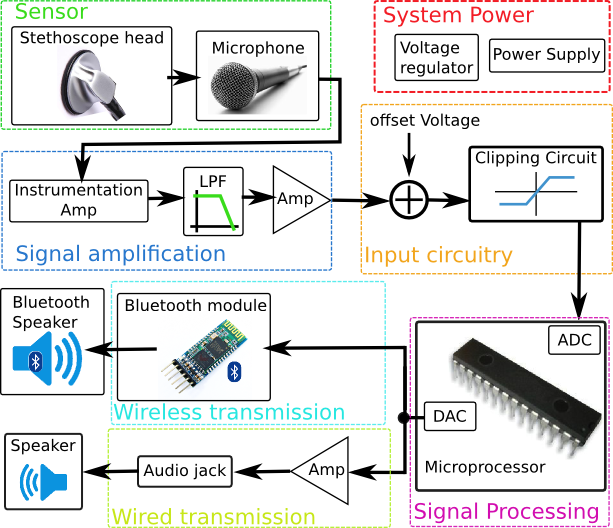
\includegraphics[resolution=120, width=315px, height=315px]{sys_overview2.png}
	
	\caption{System overview}
	\label{fig:sys_overview}
\end{figure}

The sensor consists of a conventional stethoscope head coupled to a microphone, which transforms the sound signal into a voltage signal. This signal is too small to drive any circuitry directly, so it is passed through a signal amplification stage, which results in a bipolar signal. After amplification the signal is passed through input circuitry which introduces a 1.65V offset and limits the voltage to within the maximum tolerable values of the micro-controller in the next stage. This offset is required to transform the signal from bipolar to unipolar, as the micro-controller can not read negative voltages. The micro-controller then performs signal processing in the form of a digital filter, so that it will have the same sound characteristics as a conventional stethoscope. Once processed the signal is transmitted to a Blue-tooth module which transmits the data to a Blue-tooth speaker. In addition an audio jack is available to plug in a speaker directly. All these subsystems are powered by a 9V power source, which can be switched between battery and an AC-DC wall adapter.

\section{Maximum Sound Frequency} \label{max-sound-freq}
In order to design our system we must determine what is the maximum sound frequency $f_{max}$ that it needs to measure. This frequency affects the design of the low pass filter and the sampling frequency needed for Analog to Digital Conversion. A lower $f_{max}$ results in a lower sampling frequency, which allows the microprocessor to carry out more computations per sample, and thus allows for higher order digital filters to be implemented. Higher order filters give greater flexibility in digitally manipulating the sound signal, and so would allow us to more accurately reproduce the sound characteristics of a conventional stethoscope.

An $f_{max}$ of 20kHz would work as this is the threshold of human hearing\cite[p.~163]{Stuart2011}, however it has been stated that the majority of heart and lung sounds occur at lower frequencies, within the range 37.5-1kHz\cite{Abella1992}. In order to determine $f_{max}$ 100 heart and lung sounds were analysed for their spectral content. Sound files were taken from an electronic resource used to train medical students in auscultation\cite{Coviello2014}, and three analyses were performed using MATLAB. 

The first analysis simply took a Fast Fourier Transform (FFT) of the sounds, summed the amplitudes and defined $f_{max}$ as the frequency at which this sum dropped below -80dB. In the second analysis all the sound signals were summed together, an FFT was performed on the resulting signal, and $f_{max}$ was defined to be the frequency at which the amplitude dropped below -80dB. In the third analysis the significant frequency components of each sound was calculated. Significant frequencies were defined as the range which contained 99.9\% of the signal energy, where energy is the sum of the squared FFT amplitudes. To calculate significant frequencies an iterative algorithm was used. The algorithm begins with a set that contains the signal's dominant frequency, it then adds to this set the next highest or lowest frequency, which ever has the larger FFT amplitude. The energy content of the set is compared with the energy of the sound, and the process continues until the set contains at least 99.9\% of the energy. Finally we took $f_{max}$ to be the largest frequency with at least one sound in which $f_{max}$ was considered significant. 

Analysis 1, 2, and 3 gave $f_{max}$ values 1.9kHz, 1.9kHz, and 4.0kHz respectively (Fig~\ref{fig:ausc_spectra}). If we use the most conservative result then our stethoscope needs to be able to measure and process frequencies up to at least 4.0kHz in order to capture all heart and lung sounds.

\begin{figure}[htb]
	\centering
	% \fbox{
		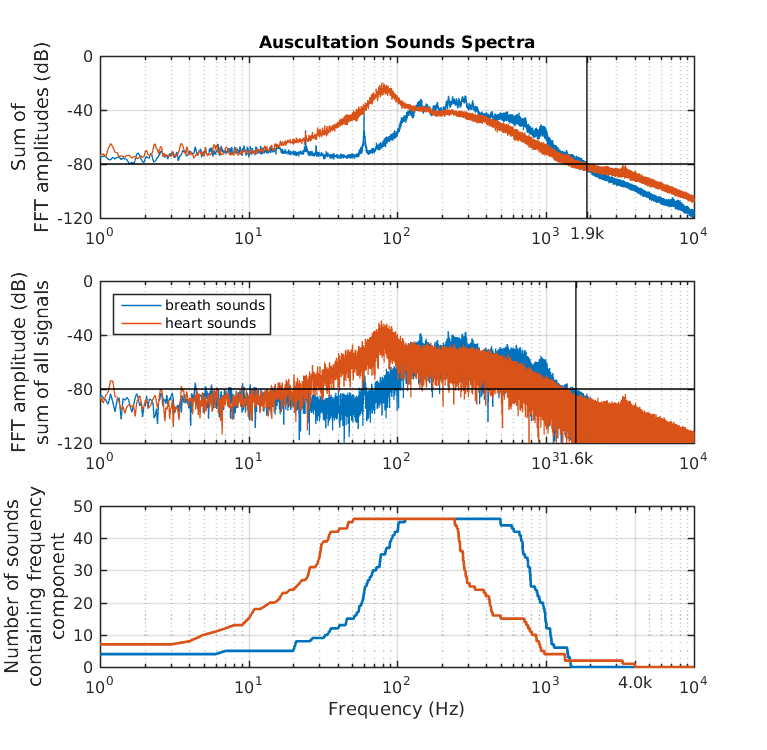
\includegraphics[width=120mm]{auscultation_spectra.png}
	% }
	\caption{Frequency spectra of auscultation sounds}
	\label{fig:ausc_spectra}
\end{figure}

\section{Signal Sensor}
Why we chose microphone vs. laser mic, vs. cap sensor \\
How we coupled microphone to stethoscope \\
Microphone circuit

\section{Signal Amplification}
\subsection{Operational Amplifiers}

Instrumentation amplifier \cite{Franco2015}
Low pass filter \cite[p.~279]{Horowitz1989}
Amplifier

\section{Input Circuitry}
DC blocker to block out any DC ofset from amplification stage\\
1.6V summing circuit to allow maximum swing\\
clipping circuit to protect 0-3.3V range \\

\section{Signal Processing}
A micro-controller processes the sound signal using Infinite Impulse Response (IIR) and Finite Impulse Response (FIR) digital filters. This signal processing is used to filter out unstable feedback frequencies and to reproduce the sound characteristics of a conventional stethoscope. Unstable feedback occurs when the microphone sensor picks up the sound played through the speaker. It happens at specific resonant frequencies which depend on the length of the coupling tube, stethoscope diaphragm, and microphone (section \ref{feedback-freq}). If left untreated these unstable frequencies can grow in amplitude until the user can only hear a large squealing sound from the device, making auscultation impossible. The micro-controller further processes the signal in order to negate the effect that having a smaller coupling tube has on the transmitted sound. The tube length of the original stethoscope is approximately 50cm, while our design has a coupling tube of only 3cm. This difference in length changes the sound transmission properties of the tube, dampening sound frequencies by a different amounts. Negating this ``colouration'' effect helps reproduce the type of sounds doctors currently listen for with a conventional stethoscope.

\subsection{Microprocessor Requirements} \label{mcu-requirements}
In order to decide which microprocessor to use we need to first establish the minimum requirements. We consider the bus size, speed, and the amount of working memory needed to implement the digital filters.

Bus sizes for microprocessors generally come in 8, 16, and 32-bit. This bus size determines the bit-depth, which is number of bits stored per sample. A larger bit-depth will require more memory to store samples, however it will suffer less quantization noise, which is the result of truncation error inherent in ADC. For our system we used 16 bit bit-depth because that's the same used in CDs~\cite[p.~27]{Schroder2011}, and we assumed CD audio quality would be sufficient.

To determine how fast the processor needs to be we estimate how many Million Instructions Per Second (MIPS) that it has to execute. To perform this calculation we need the sampling frequency ($F_s$) and the order of the digital filter we wish to implement ($N$). We take $F_s$ to be 40kHz, the Nyquist frequency associated with 20kHz sounds. Although we require to capture sounds only up to 4kHz (Section~\ref{max-sound-freq}) we use the more conservative figure for flexibility to change the design in the future. The order of the filter $N$ was unknown at the time of purchasing the micro-controller, hence an estimate of $N=100$ is used, as our past experience with designing low pass digital filters found this to be a conservative estimate. $N^{th}$ order digital filters are typically calculated as~\cite[p.~164]{Mitra2011}
\begin{equation}
y[n] = p_0 x[n] + p_1 x[n-1] + \cdots + p_N x[n-N] - d_1 y[n-1] - \cdots - d_n y[n-N]
\label{eq:filter}
\end{equation}
where $y$ is the sampled output signal, $x$ is the sampled input signal, and $d_i, p_i$ are constant filter coefficients. This requires $2N$ additions and $2N$ multiplications, for a total of $4N$ instructions per output sample $y[n]$. In addition to the digital filter the controller must also transmit 16 bits of data per sample to the Blue-tooth module, giving a required speed of $(16+4N)F_s=(16+400)40\cdot10^3=16.64$ MIPS. Thus if we round up for safety then we require a processor capable of at least 17 MIPS.

The amount of working memory required is calculated by noting that the filter in Eq.~\ref{eq:filter} needs to store $2(N+1)$ coefficients $(p_i, d_i)$, $N+1$ input signal samples $(x)$ and $N+1$ output signal samples $(y)$, for a total of $4(N+1)=404$ 16 bit values, or 808 Bytes of RAM. We round this value up to the nearest KByte and double it as a safety margin to get a minimum requirement of 2KBytes of RAM.

In summary our micro-controller needs to be at least 16-bit, capable of 17 MIPS with at least 2KBytes of working memory.

\subsection{Microprocessors Considered}
We considered five microprocessors for the system, the Arduino nano, Raspberry Pi, ADSP-BF504 Blackfin processor from Analog Devices, and the dsPIC33-FJ64GP802 from Microchip. Each processor was scored in terms of its coding, interface, size, speed, and cost, and a weighted total score determined which processor to use. 

Coding relates to what programming language the processor can be coded in. Languages such as C and Python are considered higher level than Assembly for example, and are more desirable to code in because it is quicker to develop in these languages, which will help us meet the time constraints of the project. 

Interface describes how easy it is to upload a program to the device. We wish to have the unit programmable while in a circuit in order to minimise the time it takes to debug the hardware and software. If it has to be disconnect or unplugged from our circuit for each upload iteration this could be prohibitively time consuming. 

The size of the processor will affect the size of our stethoscope. If it is too large to be comfortably held in the hand then it will not have met its specifications, thus we require a processor that won't greatly increase the size of our final design.

Speed is constrained to be at least 17 MIPS (Section~\ref{mcu-requirements}), anything above this is considered a bonus as it allows for further flexibility in filter design. 

Finally we considered cost, by minimising the processor cost we minimise the cost of our final device and thus the likelihood of it being used or purchased.

From our weighted total scores we decided to use the dsPIC33-FJ64GP802 microprocessor (Table~\ref{mcu-decision-matrix}). In our scoring analysis we estimated the speed to be the clock frequency of the device, which meant the Adruino was not fast enough to perform the required filtering computation. The Raspberry pi provided the greatest speed however it was both the largest and most expensive option, which made it less feasible. The Blackfin BF504 also provided considerable speed however it was only sold in surface mount packages or as part of a development board, making it difficult to prototype onto a bread board. Thus because of its low cost, small form factor, and ability to handle the required computation we decided to use the dsPIC.
\begin{table}[htbp]
\caption{Microcontroller decision matrix}
\begin{center}
\begin{tabular}{rccccc}

\hline
\multirow{2}{*}{\textbf{}} & 
\multirow{2}{*}{\textbf{weight}} & 
\textbf{\small{Arduino}} & 
\textbf{\small{Raspberry}} & 
\textbf{\small{AD}} & 
\multirow{2}{*}{\textbf{\small{dsPIC}}} \\ 


 & & \textbf{\small{(nano)}} & \textbf{\small{pi}} & \textbf{\small{Blackfin}} & \\

\hline

\textbf{Coding} & 7 & 10 & 10 & 10 & 10 \\ \hline

\textbf{Interface} & 10 & 10 & 10 & 1  & 10 \\
& & \multicolumn{2}{c}{\small{(USB cable)}} & \small{(dev board / SMD)} & \small{(programmer)} \\
\hline

\textbf{Size} & 9 & 7 & 5 & 10 & 10 \\
& & \small{(3cm$\times$5cm)} & \small{(10cm$\times$15cm)} & \small{(1.2cm$\times$1.2cm)} & \small{(0.7cm$\times$3.6cm)} \\
\hline
 
\textbf{Speed} & 6 & 0 & 10 & 9 & 7 \\
& & \small{(16MIPS)} & \small{(700MIPS)} & \small{(400MIPS)} & \small{(40MIPS)} \\
\hline

\textbf{Cost} & 8 & 6 & 4 & 5 & 10 \\ 
& & \small{(\$20)} & \small{(\$30)} & \small{(\$25)} & \small{(\$5)}\\
\hline

\multicolumn{2}{r}{\textbf{\footnotesize{Total weighted score}}} & \textbf{281} & \textbf{307} & \textbf{264} & \textbf{382} \\ \hline
\end{tabular}
\end{center}
\label{mcu-decision-matrix}
\end{table}


\subsection{dsPIC33 micro-controller}
\subsubsection{Features}
We used a dsPIC33-FJ64GP802 microprocessor to process the sound signal. The chip contains an ADC, audio DAC and dedicated Digital Signal Processing (DSP) engine, which make it well suited to filter our signal. The DSP engine (Fig.~\ref{fig:dsp_block}) is capable of retrieving two words of data from memory, multiplying them and summing them to a running total in a single instruction cycle. This operation of Multiplying and ACcumulating (MAC) is frequently used in digital filters, and so being able to perform a MAC in a single cycle makes the chip efficient for our purposes. The ADC is capable of converting 500k 12-bit samples per second through successive approximation conversion, so it is fast enough to handle our maximum requirement of 40k samples per second. ADC conversions are also written directly to memory, without any CPU intervention, through the chip's Direct Memory Access (DMA) feature, resulting in less overhead and allowing the chip to execute more instructions per sample. Finally the DAC is designed specifically for audio applications, and is capable of producing up to 40kHz signals, making it suitable for our application as we wish to output a filtered sound signal. 

\begin{figure}[!ht]
	\centering
	% \fbox{
		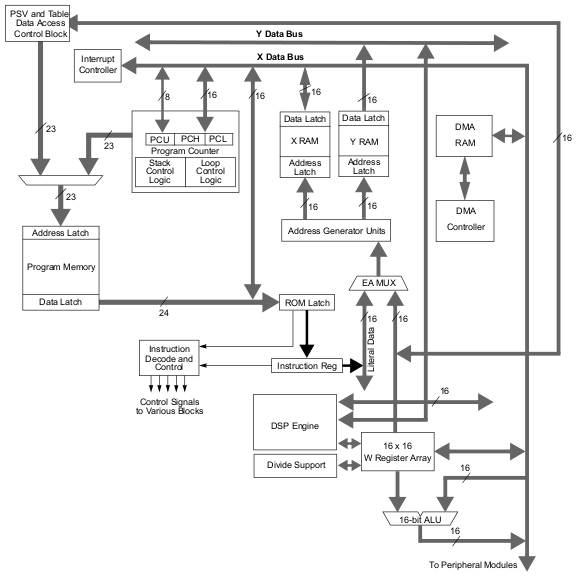
\includegraphics[width=110mm]{dsp_engine.png}
	% }
	\caption{Micro-controller block diagram, taken from dsPIC33 data-sheet \cite[p.~14]{dspic_datasheet}}
	\label{fig:dsp_block}
\end{figure}

\subsubsection{Operation}
The dsPIC utilises two memory locations, buffers A and B, to apply the digital filter. In one cycle the ADC writes to buffer A, while the filter function operates on data in buffer B and outputs the result to the DAC (Figure~\ref{fig:mcu_operation}). In the next cycle the ADC writes to buffer B while the filter is applied to buffer A samples. This ``ping-pong'' switching between the two buffers allows the ADC to sample data while the dsPIC simultaneously applies a digital filter to previous data samples, which results in a continuously filtered output signal. The filter is executed using the IIR and FIR functions of the DSP library that is included with Microchip's dsPIC Integrated Development Environment ``MPLABX''.

It is important to assure that the rate at which buffer's A and B are written to by the ADC and read from by the DAC are synchronized, otherwise the output signal will be distorted. If the ADC writes data at a different rate than the DAC reads it then the output signal will be shifted in frequency compared to the input signal. It is also possible for newer input samples to overwrite previous ones before they've been processed, corrupting that block of data. The time at which the ADC samples is controlled by an internal counter. The counter raises an interrupt after a programmed number of system clock cycles, which gives us great flexibility in setting the ADC sampling frequency. The DAC clock however is constrained to run off an auxiliary clock, scaled down by a selectable factor from between 1 to 128, which restricts what sampling frequencies we can use the most.

\begin{figure}[!htb]
	\centering
	% \fbox{
		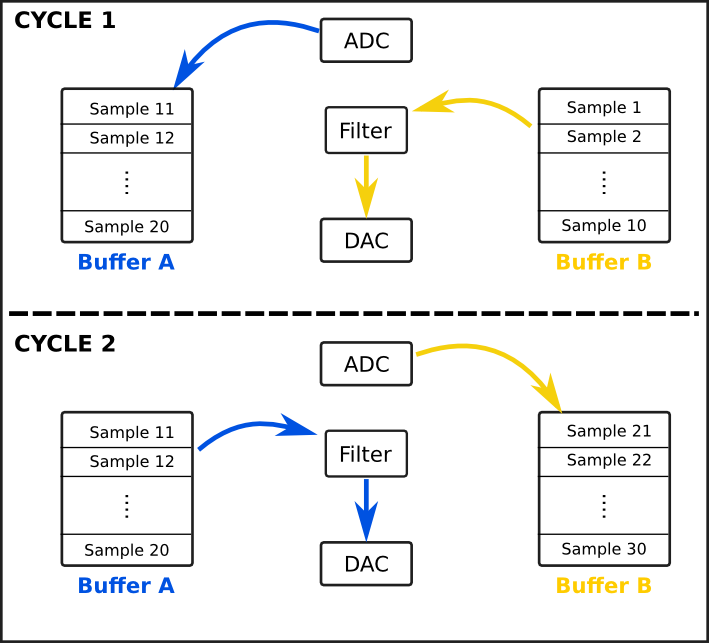
\includegraphics[width=90mm]{mcu_operation.png}
	% }
	\caption{Micro-controller sampling and filtering process}
	\label{fig:mcu_operation}
\end{figure}



\section{Wireless Transmission}
Yudong

\section{Wired Transmission}
Yudong

\section{System Power}
Yudong